\chapter{Hypothetischer Patentantrag\label{cha:chapter5}}

\section{Vorbereitung der Patentanmeldung}

Um ein Patent beim DPMA Anzumelden wird ein Anmeldeformular benötigt (Formular P 2790),
welches im Internet unter \url{https://www.dpma.de/docs/formulare/patent/p2007.pdf} heruntergeladen
werden kann. 
Eine ausschließlich Windows kompatible Alternative bietet
das DPMA direktPro-System zur Online Anmeldung von Patenten.

Das Anmeldeformular verlangt:

\begin{enumerate}
    \item Angaben zum Anmelder
    \item Erfindernennung (falls abweichend vom Anmelder)
    \item Titel der Erfindung, Art der Erfindung
    \item Prioritätsangaben (falls in mehreren Ländern eingereicht)
    \item Angaben zu den Unterlagen (beigefügte Dokumente)
    \item Wahl des Prüfungsverfahrens (inhaltliche Prüfung des Antrags)
	\item Zahlungsweise
\end{enumerate}

Dabei ist zu beachten, das die Wahl des Prüfungsverfahrens 
(Rechercheantrag (§ 43 Patentgesetz)) oder
Prüfungsantrag (§ 44 Patentgesetz) zusätzliche einmalige Kosten verursacht.
Bei Auslassen der Wahl des Prüfungsverfahrens wird eine rein formulare
Prüfung des Patentantrages durchgeführt und keine inhaltliche.
Erfolgt lediglich eine Formalprüfung wird das Patent nicht erteilt.
Weitere Bestandteile der Patentanmeldung sind laut DPMA \cite{DPMAAnmeldung}:

\begin{enumerate}
	\item Technische Beschreibung der Erfindung, gegebenenfalls mit Bezugszeichenliste
	\item Patentansprüche
	\item Zeichnungen, falls von Ihnen als notwendig erachtet
	\item Zusammenfassung
	\item Erfinderbenennung
\end{enumerate}

Diese Dokumente werden mit dem Punkt Angaben 
zu den Unterlagen (beigefügte Dokumente) abgedeckt.

\section{Erstellung KI-Patent}

Um eine durch KI entwickelte Erfindung zu generieren, 
welche relativ wenig durch den Input beeinflusst wurde, 
wird der Input:
"Erstelle eine patentierbare technische Erfindung 
in Form eines Computerprogrammes im Bereich Iot" in ChatGPT-4o eingegeben.
Die daraus entstandene Erfindung lautet:
Intelligentes Energiemanagementsystem für \gls{IoT}-basierte Haushalte.
Als Anmelder tritt wie in Kapitel 3 durch den BGH festgelegt der Benutzer
der KI in Erscheinung \ref{cha:chapter3} \ref{fig:Pat1-3}.
\begin{figure}[htb]
    \centering
    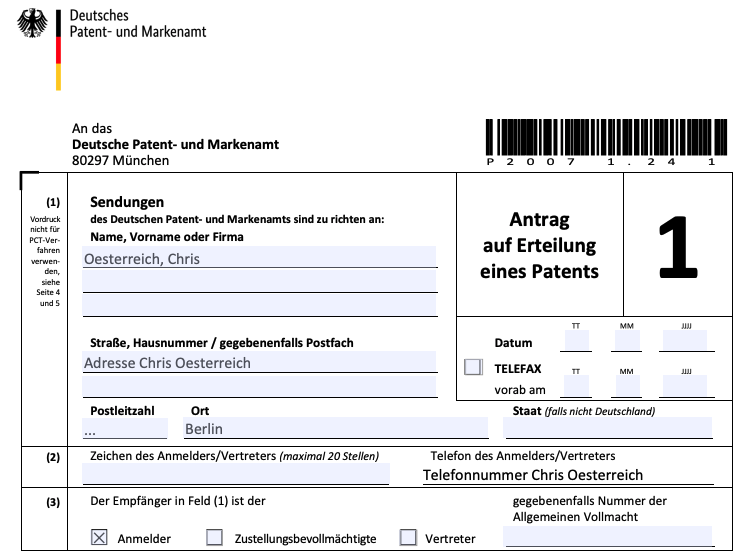
\includegraphics[width=\textwidth]{Patentanmeldung1-3.png}\\
    \caption{ Patentanmeldung Schritte 1-3 }\label{fig:Pat1-3}
\end{figure}
\\
Damit sind die Punkte "Angaben zum Anmelder" und "Erfindernennung" bearbeitet, 
da der Erfinder hier gleich dem Anmelder ist.
Die Bezeichnung der Erfindung ist:
Intelligentes Energiemanagementsystem für IoT-basierte Haushalte.
Die hypothetische Patentanmeldung soll sowohl einen Prüfungsantrag, 
als auch einen Rechercheantrag beinhalten \ref{fig:Pat6-7}.
\begin{figure}[htb]
    \centering
    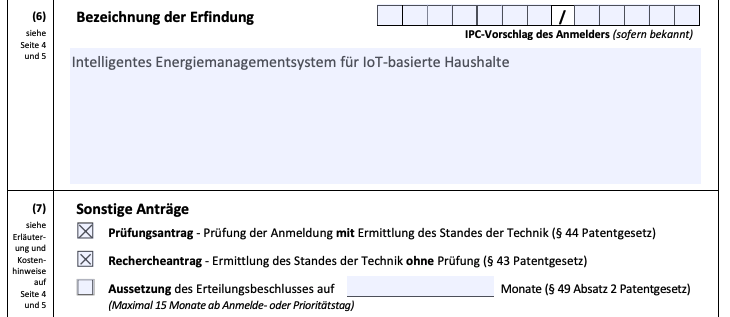
\includegraphics[width=\textwidth]{Patentanmeldung6-7.png}\\
    \caption{ Patentanmeldung Schritte 6-7 }\label{fig:Pat6-7}
\end{figure}
\\
\\
Für den Rechercheantrag fällt eine Gebühr von 300 Euro an (Stand 2024),
für den Prüfungsantrag 150 Euro, in Kombination mit dem Rechercheantrag (Stand 2024).
Bei Anmeldung in Papierform bis zu 10 Patentansprüche fällt außerdem noch eine
Anmeldegebühr von 60 Euro an (Stand 2024). Bei jedem weiteren Anspruch
fallen 30 Euro pro Anspruch an(Stand 2024) Dies ergibt für das obige Patent 
eine Anmeldegebühr von 570 Euro \ref{fig:Pat10}.
\begin{figure}[htb]
    \centering
    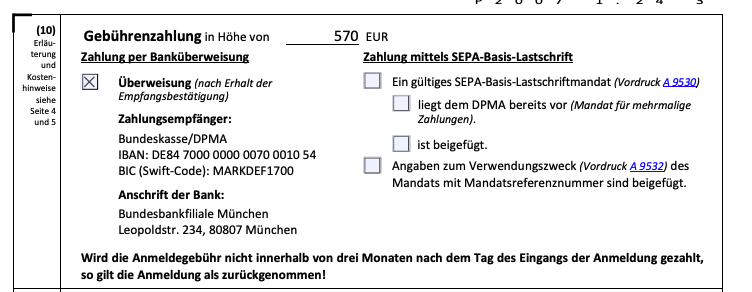
\includegraphics[width=\textwidth]{Patentanmeldung10.png}\\
    \caption{ Patentanmeldung Schritte 10 }\label{fig:Pat10}
\end{figure}

Für die oben geforderten Anlagen sind mehr Informationen von der KI
bezüglich des Patents nötig.

Als Beschreibung der Erfindung \ref{beschPDF} gibt ChatGPT-4o eine Einordnung 
in das Technische Gebiet, den Stand der Technik, die Problemlösung,
die technischen Merkmale , sowie Vorteile der Erfindung zurück.
Patentansprüche \ref{schutzPDF} 
und eine Zusammenfassung \ref{zusammenfassungPDF} müssen in zusätzlichen Prompts 
abgefragt werden. 
Damit wären die Grundbestandteile der Patentanmeldung erfüllt und nach Angabe der 
Zahlungsweise und
Einreichung der Anmeldung beim DPMA würde die Prüfung beginnen. 

\section{Die von der KI entwickelte Erfindung}


\section{Prüfung der KI Erfindung}
Die von ChatGPT-4o entstandene Erfindung nutzt machinelles lernen um eine effiziente
Energieverwaltung in Haushalten zu ermöglichen. 




